\section{peo\-EA$<$ EOT $>$ Class Template Reference}
\label{classpeo_e_a}\index{peoEA@{peoEA}}
The {\bf peo\-EA}{\rm (p.\,\pageref{classpeo_e_a})} class offers an elementary evolutionary algorithm implementation.  


{\tt \#include $<$peo\-EA.h$>$}

Inheritance diagram for peo\-EA$<$ EOT $>$::\begin{figure}[H]
\begin{center}
\leavevmode
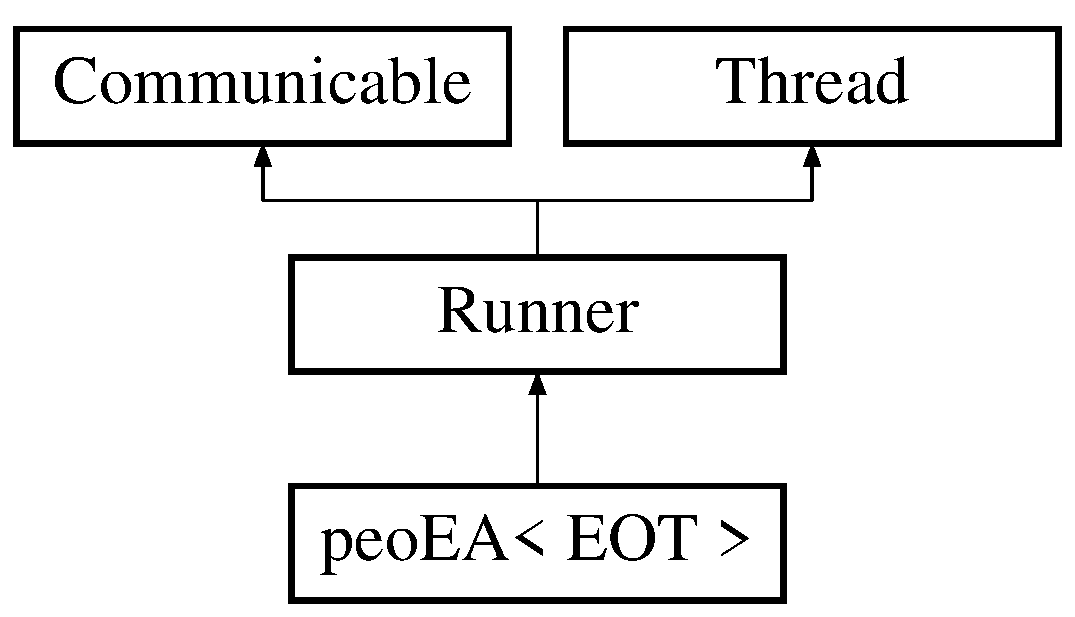
\includegraphics[height=3cm]{classpeo_e_a}
\end{center}
\end{figure}
\subsection*{Public Member Functions}
\begin{CompactItemize}
\item 
{\bf peo\-EA} (eo\-Continue$<$ EOT $>$ \&\_\-\_\-cont, {\bf peo\-Pop\-Eval}$<$ EOT $>$ \&\_\-\_\-pop\_\-eval, eo\-Select$<$ EOT $>$ \&\_\-\_\-select, {\bf peo\-Transform}$<$ EOT $>$ \&\_\-\_\-trans, eo\-Replacement$<$ EOT $>$ \&\_\-\_\-replace)
\begin{CompactList}\small\item\em Constructor for the evolutionary algorithm object - several basic parameters have to be specified, allowing for different levels of parallelism. \item\end{CompactList}\item 
void {\bf run} ()\label{classpeo_e_a_6ab8c321d29350634143a2a01cf2ad24}

\begin{CompactList}\small\item\em Evolutionary algorithm function - a side effect of the fact that the class is derived from the {\bf {\bf Runner}{\rm (p.\,\pageref{class_runner})}} class, thus requiring the existence of a {\em run\/} function, the algorithm being executed on a distinct thread. \item\end{CompactList}\item 
void {\bf operator()} (eo\-Pop$<$ EOT $>$ \&\_\-\_\-pop)
\begin{CompactList}\small\item\em Function operator for specifying the population to be associated with the algorithm. \item\end{CompactList}\end{CompactItemize}
\subsection*{Private Attributes}
\begin{CompactItemize}
\item 
eo\-Continue$<$ EOT $>$ \& {\bf cont}\label{classpeo_e_a_5f015eebf42f176b9fe322488c446c2a}

\item 
{\bf peo\-Pop\-Eval}$<$ EOT $>$ \& {\bf pop\_\-eval}\label{classpeo_e_a_9140259f50c9186edcb062b023624c96}

\item 
eo\-Select$<$ EOT $>$ \& {\bf select}\label{classpeo_e_a_2d8428d69fdd6aefefbaf543fdd46d19}

\item 
{\bf peo\-Transform}$<$ EOT $>$ \& {\bf trans}\label{classpeo_e_a_713c77935eb8aafebfb9488cfaa4a363}

\item 
eo\-Replacement$<$ EOT $>$ \& {\bf replace}\label{classpeo_e_a_9bd2d4356cf7e69e3141dc269213aa8a}

\item 
eo\-Pop$<$ EOT $>$ $\ast$ {\bf pop}\label{classpeo_e_a_c0b110e410bc16283e8339f24b733772}

\end{CompactItemize}


\subsection{Detailed Description}
\subsubsection*{template$<$class EOT$>$ class peo\-EA$<$ EOT $>$}

The {\bf peo\-EA}{\rm (p.\,\pageref{classpeo_e_a})} class offers an elementary evolutionary algorithm implementation. 

In addition, as compared with the algorithms provided by the EO framework, the {\bf peo\-EA}{\rm (p.\,\pageref{classpeo_e_a})} class has the underlying necessary structure for including, for example, parallel evaluation and parallel transformation operators, migration operators etc. Although there is no restriction on using the algorithms provided by the EO framework, the drawback resides in the fact that the EO implementation is exclusively sequential and, in consequence, no parallelism is provided. A simple example for constructing a {\bf peo\-EA}{\rm (p.\,\pageref{classpeo_e_a})} object:

\begin{TabularC}{2}
\hline
... ~ &~  \\\hline
eo\-Pop$<$ EOT $>$ population( POP\_\-SIZE, pop\-Initializer ); ~ &// creation of a population with POP\_\-SIZE individuals - the pop\-Initializer is a functor to be called for each individual \\\hline
~  &~  \\\hline
eo\-Gen\-Continue$<$ EOT $>$ ea\-Cont( NUM\_\-GEN ); ~ &// number of generations for the evolutionary algorithm \\\hline
eo\-Check\-Point$<$ EOT $>$ ea\-Checkpoint\-Continue( ea\-Cont ); ~ &// checkpoint incorporating the continuation criterion - startpoint for adding other checkpoint objects \\\hline
~  &~  \\\hline
peo\-Seq\-Pop\-Eval$<$ EOT $>$ ea\-Pop\-Eval( eval\-Function ); ~ &// sequential evaluation functor wrapper - eval\-Function represents the actual evaluation functor  \\\hline
~  &~  \\\hline
eo\-Ranking\-Select$<$ EOT $>$ selection\-Strategy; ~ &// selection strategy for creating the offspring population - a simple ranking selection in this case  \\\hline
eo\-Select\-Number$<$ EOT $>$ ea\-Select( selection\-Strategy, POP\_\-SIZE ); ~ &// the number of individuals to be selected for creating the offspring population  \\\hline
eo\-Ranking\-Select$<$ EOT $>$ selection\-Strategy; ~ &// selection strategy for creating the offspring population - a simple ranking selection in this case  \\\hline
~  &~  \\\hline
eo\-SGATransform$<$ EOT $>$ transform( crossover, CROSS\_\-RATE, mutation, MUT\_\-RATE ); ~ &// transformation operator - crossover and mutation operators with their associated probabilities  \\\hline
peo\-Seq\-Transform$<$ EOT $>$ ea\-Transform( transform ); ~ &// Paradis\-EO specific sequential operator - a parallel version may be specified in the same manner  \\\hline
~  &~  \\\hline
eo\-Plus\-Replacement$<$ EOT $>$ ea\-Replace; ~ &// replacement strategy - for integrating the offspring resulting individuals in the initial population  \\\hline
~  &~  \\\hline
peo\-EA$<$ EOT $>$ ea\-Alg( ea\-Checkpoint\-Continue, ea\-Pop\-Eval, ea\-Select, ea\-Transform, ea\-Replace ); ~ &// Paradis\-EO evolutionary algorithm integrating the above defined objects  \\\hline
ea\-Alg( population ); ~ &// specifying the initial population for the algorithm  \\\hline
... ~ &~  \\\hline
\end{TabularC}




Definition at line 69 of file peo\-EA.h.

\subsection{Constructor \& Destructor Documentation}
\index{peoEA@{peo\-EA}!peoEA@{peoEA}}
\index{peoEA@{peoEA}!peoEA@{peo\-EA}}
\subsubsection{\setlength{\rightskip}{0pt plus 5cm}template$<$class EOT$>$ {\bf peo\-EA}$<$ EOT $>$::{\bf peo\-EA} (eo\-Continue$<$ EOT $>$ \& {\em \_\-\_\-cont}, {\bf peo\-Pop\-Eval}$<$ EOT $>$ \& {\em \_\-\_\-pop\_\-eval}, eo\-Select$<$ EOT $>$ \& {\em \_\-\_\-select}, {\bf peo\-Transform}$<$ EOT $>$ \& {\em \_\-\_\-trans}, eo\-Replacement$<$ EOT $>$ \& {\em \_\-\_\-replace})}\label{classpeo_e_a_dbfc4f8907bef234602149229f132371}


Constructor for the evolutionary algorithm object - several basic parameters have to be specified, allowing for different levels of parallelism. 

Depending on the requirements, a sequential or a parallel evaluation operator may be specified or, in the same manner, a sequential or a parallel transformation operator may be given as parameter. Out of the box objects may be provided, from the EO package, for example, or custom defined ones may be specified, provided that they are derived from the correct base classes.

\begin{Desc}
\item[Parameters:]
\begin{description}
\item[{\em eo\-Continue$<$}]EOT $>$\& \_\-\_\-cont - continuation criterion specifying whether the algorithm should continue or not; \item[{\em peo\-Pop\-Eval$<$}]EOT $>$\& \_\-\_\-pop\_\-eval - evaluation operator; it allows the specification of parallel evaluation operators, aggregate evaluation functions, etc.; \item[{\em eo\-Select$<$}]EOT $>$\& \_\-\_\-select - selection strategy to be applied for constructing a list of offspring individuals; \item[{\em peo\-Transform$<$}]EOT $>$\& \_\-\_\-trans - transformation operator, i.e. crossover and mutation; allows for sequential or parallel transform; \item[{\em eo\-Replacement$<$}]EOT $>$\& \_\-\_\-replace - replacement strategy for integrating the offspring individuals in the initial population; \end{description}
\end{Desc}


Definition at line 113 of file peo\-EA.h.

References peo\-EA$<$ EOT $>$::pop\_\-eval, and peo\-EA$<$ EOT $>$::trans.

\subsection{Member Function Documentation}
\index{peoEA@{peo\-EA}!operator()@{operator()}}
\index{operator()@{operator()}!peoEA@{peo\-EA}}
\subsubsection{\setlength{\rightskip}{0pt plus 5cm}template$<$class EOT$>$ void {\bf peo\-EA}$<$ EOT $>$::operator() (eo\-Pop$<$ EOT $>$ \& {\em \_\-\_\-pop})}\label{classpeo_e_a_3c709e3b2491147d26fee36138644613}


Function operator for specifying the population to be associated with the algorithm. 

\begin{Desc}
\item[Parameters:]
\begin{description}
\item[{\em eo\-Pop$<$}]EOT $>$\& \_\-\_\-pop - initial population of the algorithm, to be iteratively evolved; \end{description}
\end{Desc}


Definition at line 129 of file peo\-EA.h.

References peo\-EA$<$ EOT $>$::pop.

The documentation for this class was generated from the following file:\begin{CompactItemize}
\item 
peo\-EA.h\end{CompactItemize}
